\section{Konjunktur}
\subsection{Der negative Nachfrageschock}
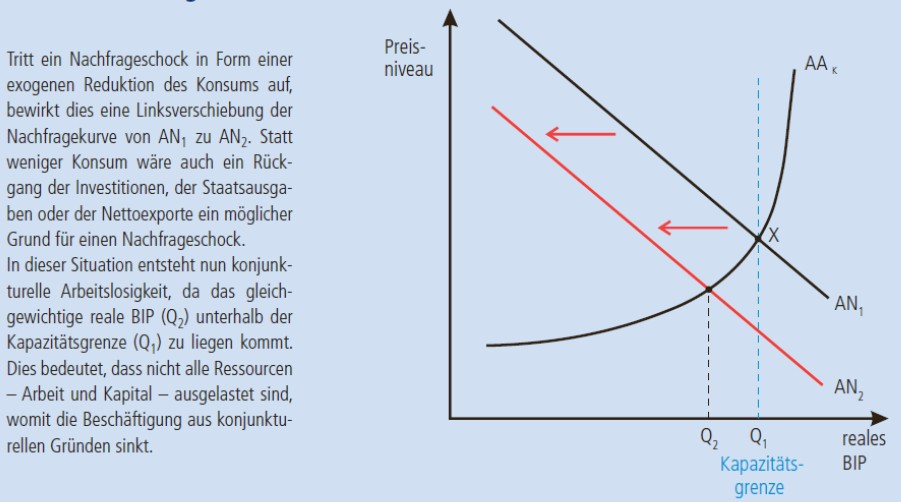
\includegraphics[width=0.9\linewidth]{images/negnach.jpg}
\subsection{Der kurzfristige positive Nachfrageschock}
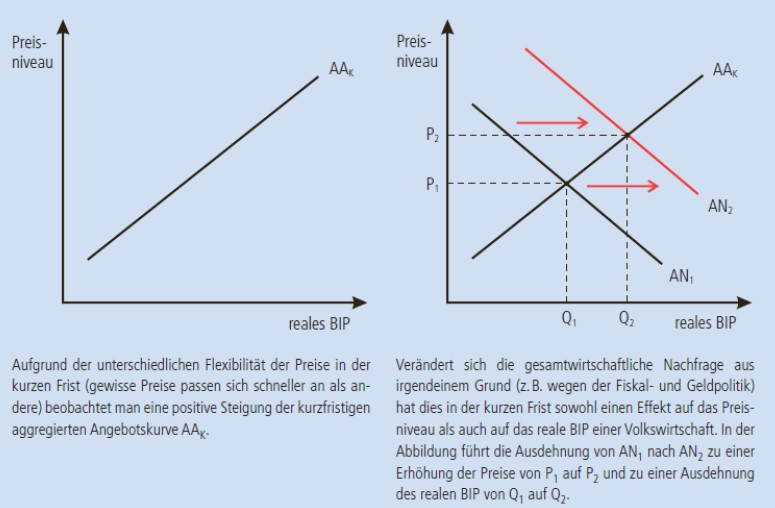
\includegraphics[width=0.9\linewidth]{images/posnachkurz.jpg}
\subsection{Der langfristige positive Nachfrageschock}
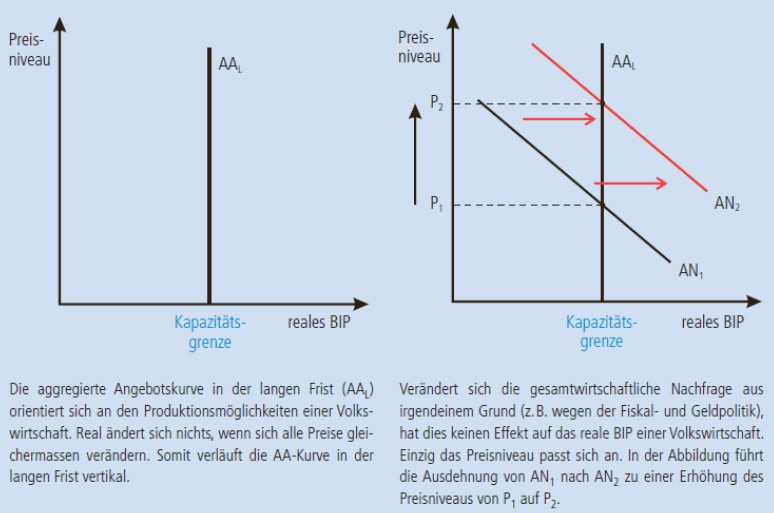
\includegraphics[width=0.9\linewidth]{images/posnachlang.jpg}
\subsection{Der negative Angebotsschock}
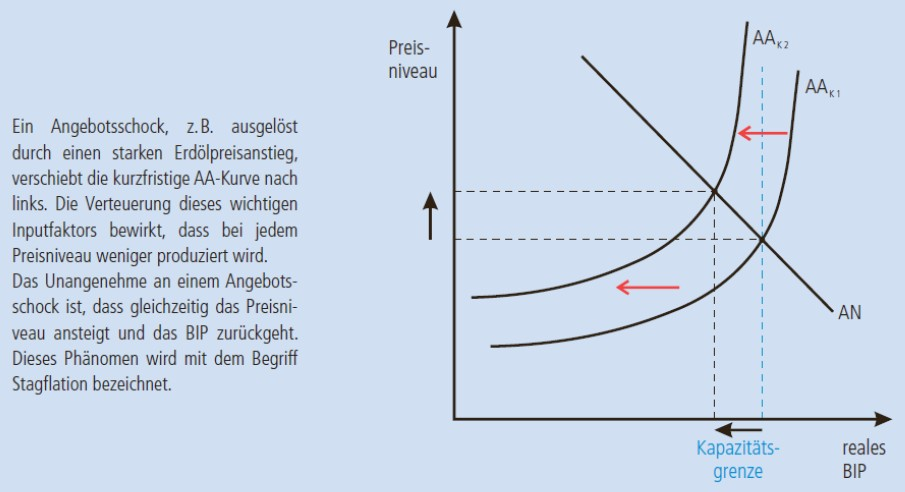
\includegraphics[width=0.9\linewidth]{images/negangebot.jpg}
\subsection{Der positive Angebotsschock}
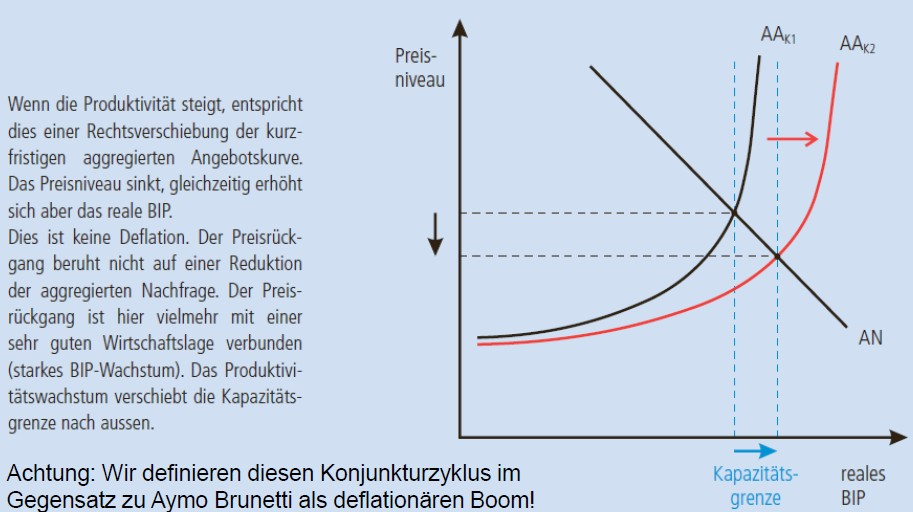
\includegraphics[width=0.9\linewidth]{images/posangebot.jpg}
\subsection{Konjunkturzyklen}
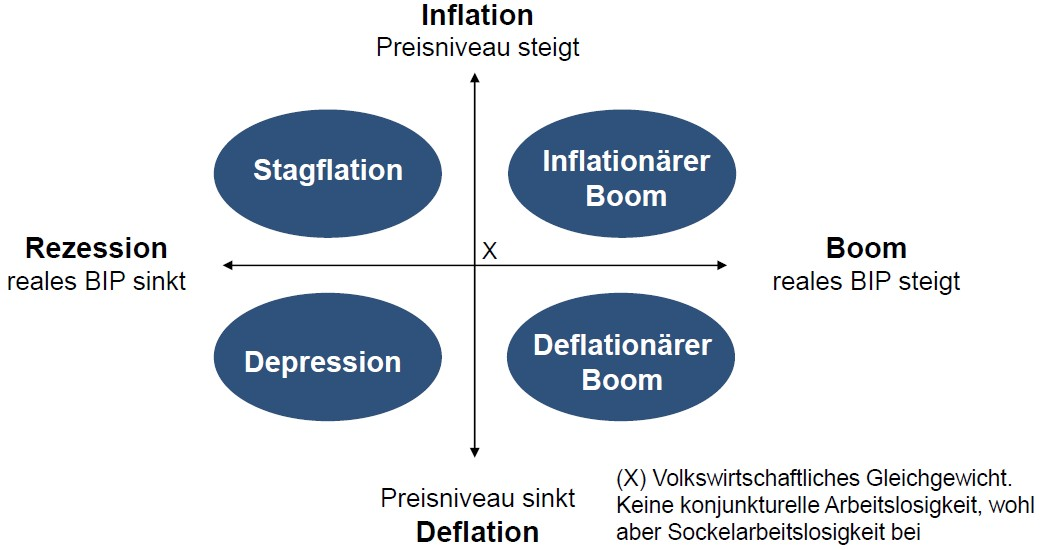
\includegraphics[width=0.9\linewidth]{images/konjukturzyklen.jpg}\\
Durch die Konjunkturzyklen entsteht konjunkturelle Arbeitslosigkeit. Diese wird mit der Konjunkturpolitik bekämpft. Diese Politik gibt es in drei Formen.\\
\begin{minipage}{11cm}
	\begin{itemize}
		\item \textbf{1.Nichts tun} 
		\subitem Anpassung ohne aktive Konjunkturpolitik
		\subitem Automatisches Wiederherstellen auf lange Sicht
		\subitem Gleiches BIP aber tieferes Preisniveau		
	\end{itemize}
\end{minipage}
\begin{minipage}{8cm}
	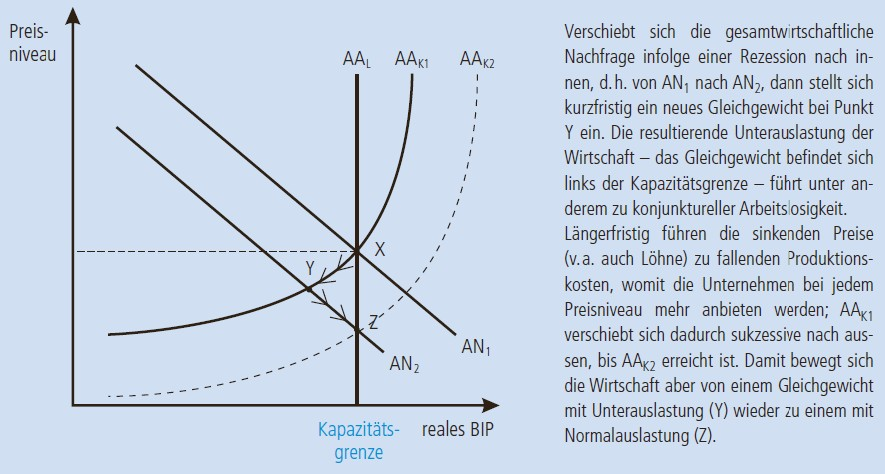
\includegraphics[width=8cm]{images/nichts.jpg}
\end{minipage}
\begin{minipage}{11cm}
	\begin{itemize}
		\item \textbf{2.Aktive keynesianische Konjukturpolitik}
		\subitem Positiver Schock auf Nachfrageseite
		\subitem Staat fördert durch Fiskal- und Geldpolitik
		\subitem Problem der Wirkungsverzögerung
	\end{itemize}
\end{minipage}
\begin{minipage}{8cm}
	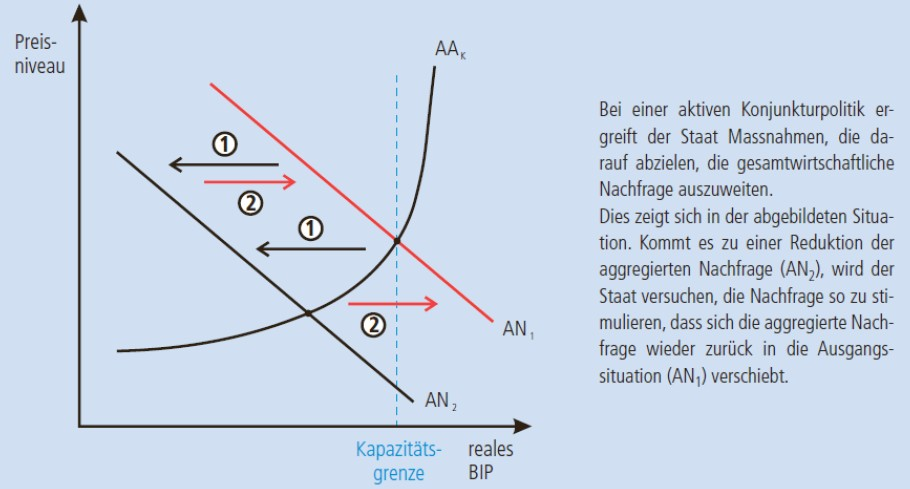
\includegraphics[width=8cm]{images/keyne.jpg}
\end{minipage}
\begin{minipage}{11cm}
	\begin{itemize}
		\item \textbf{3.Stärkung automatische Stabilisatoren}
		\subitem Staatliche Einnahmen und Ausgaben dass automatisch Nachfrage stimuliert werden
		\subitem Steuern, Schuldenbremse, Arbeitslosenversicherung
	\end{itemize}
\end{minipage}
\begin{minipage}{8cm}
	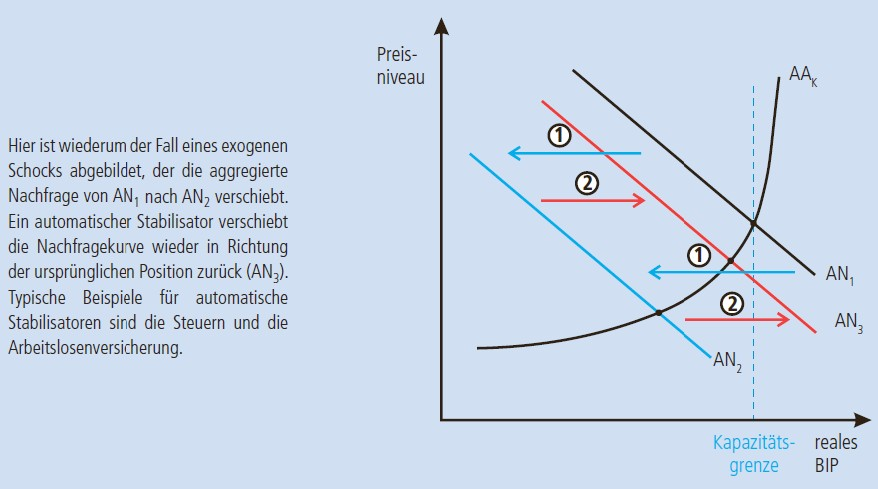
\includegraphics[width=8cm]{images/autostab.jpg}
\end{minipage}
